\section{Diskussion}
\label{sec:Diskussion}

\subsection{Lange Spule}

Es wird eine Abweichung von 283 \% der Theoriewerte zu den Messwerten beobachtet. Grund hierfür könnte
eine falsch angegebene Windungszahl, Radius der Spule oder auch ein Fehler des Konstanters. Wenn das Strom-
Messgerät falsche Werte für den Strom anzeigt, kann dieser auch nicht genau eingestellt werden und führt
so zu größeren Abweichungen.\\
Zudem war die Messvorrichtung sehr wackelig und ungenau, da ein loses Holz-Lineal als Messgerät verwendet wurde.
Eine weitere mögliche Fehlerquelle ist die sehr empfindliche Hall-Sonde, welche durch das Anfängerpraktikum sehr
viel von unerfahrenen Studenten benutzt wird und dadurch kaputt gehen kann.

\subsection{Helmholtz-Spulenpaar}

Bei jedem gewählten Abstand $a$ waren die Abweichungen zu den Theoriewerten sehr gering (11,24 \%, 13,26 \% und 15,67 \%).
Die Messung verlief reibungslos und konnte mit guter Präzission durchgeführt werden. Mögliche Fehlerquelle
wäre hier wieder die Genauigkeit des Stroms oder Fehler der Hall-Sonde.

\subsection{Hysteresekurve}

Die Messwerte passen alle gut und die wichtigen Punkte lassen sich gut ablesen. Es gibt keine Theoriewerte zum
vergleichen.

\section{Messwerte}

\label{sec:Messwerte}

\begin{figure}
  \centering
  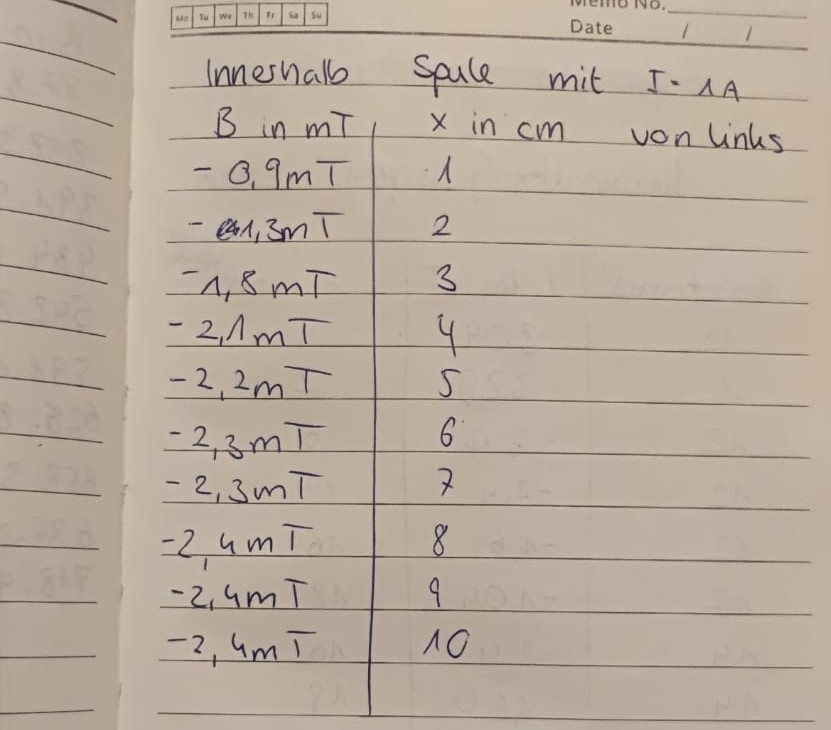
\includegraphics[width=0.7\textwidth]{Spule.jpeg}
  \caption{Messwerte der langen Spule.}
  \label{fig:M1}
\end{figure}
\begin{figure}
    \centering
    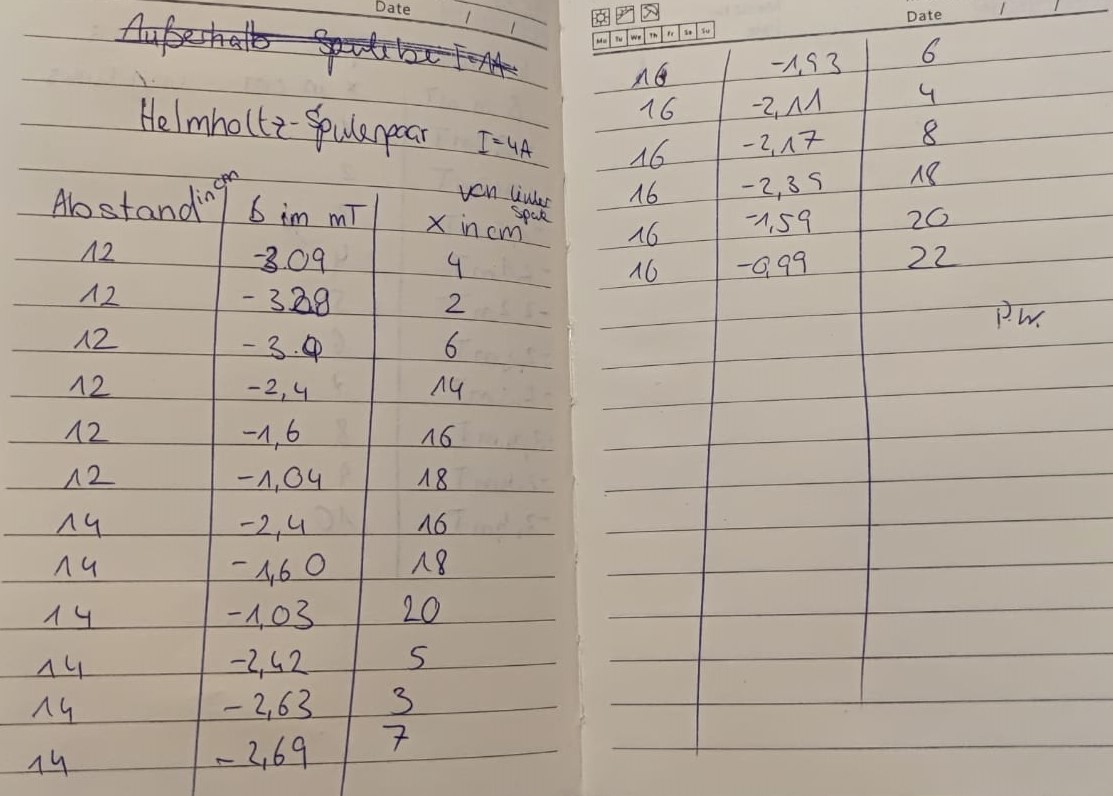
\includegraphics[width=0.7\textwidth]{Helm.jpeg}
    \caption{Messwerte des Helmholtz-Spulenpaars.}
    \label{fig:M2}
\end{figure}
\begin{figure}
    \centering
    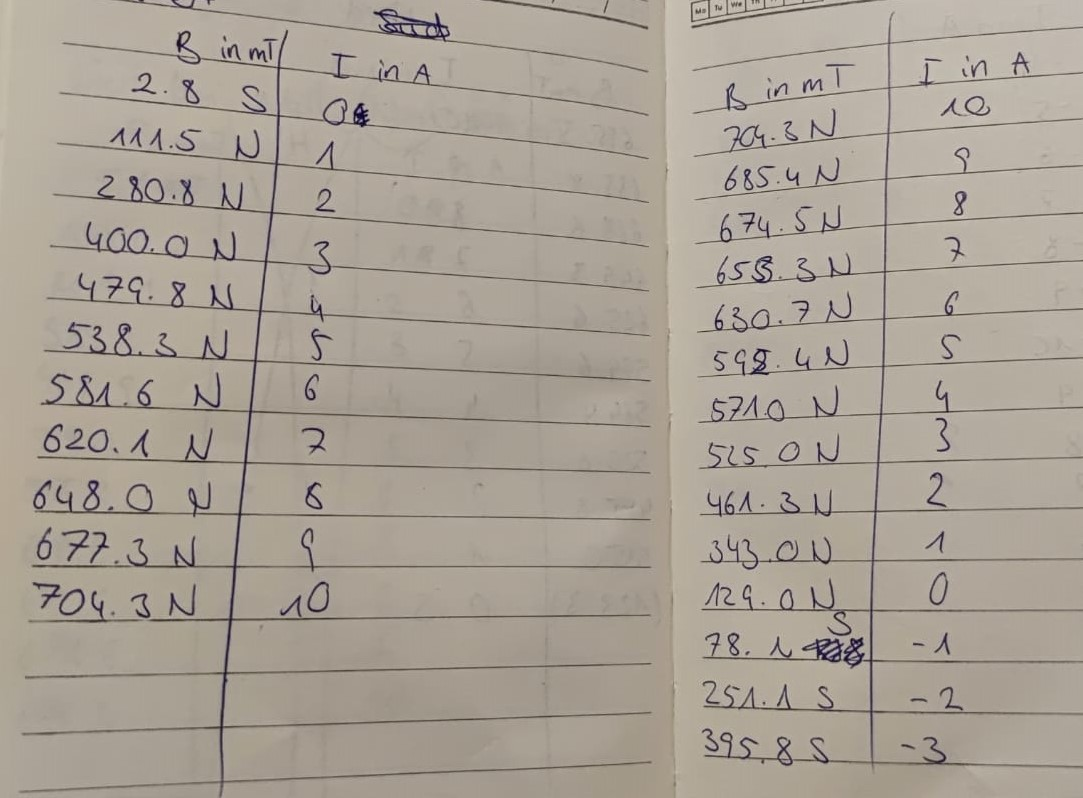
\includegraphics[width=0.7\textwidth]{Ring1.jpeg}
    \caption{Messwerte der Ringspule No1.}
    \label{fig:M3}
\end{figure}
\begin{figure}
    \centering
    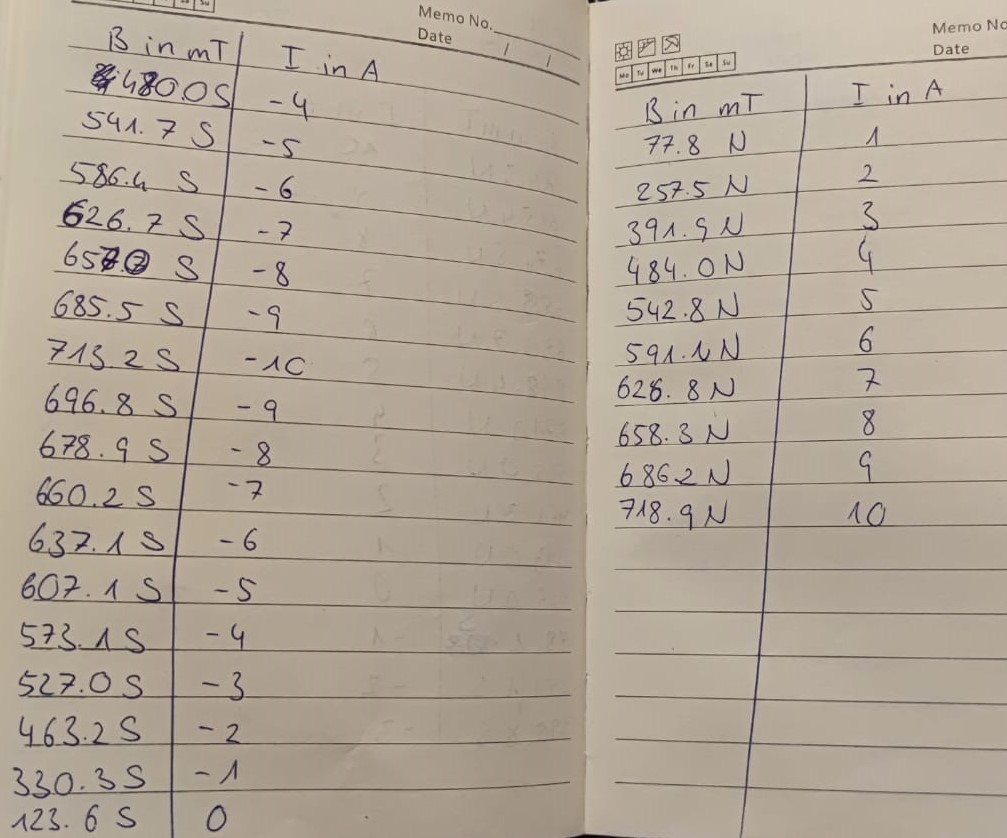
\includegraphics[width=0.7\textwidth]{Ring2.jpeg}
    \caption{Messwerte der Ringspule No2.}
    \label{fig:M4}
\end{figure}